\documentclass[12pt]{article}
\usepackage[english]{babel}
\usepackage[utf8x]{inputenc}
\usepackage{amsmath}
\usepackage{graphicx}
\usepackage{booktabs}
\usepackage{float}
\usepackage[colorinlistoftodos]{todonotes}
\usepackage{epstopdf}
\usepackage[margin=1.0in]{geometry}
\usepackage{hyperref, caption}

% Source code formating
\usepackage{listings}
\lstset{ 
 %frame=single,
 language=Verilog,
 %numbers=left,
 breaklines=true,
  basicstyle=\small, %or \small or \footnotesize etc.
 title=\lstname
}


\begin{document}

\begin{titlepage}

\newcommand{\HRule}{\rule{\linewidth}{0.5mm}} % Defines a new command for the horizontal lines, change thickness here

\center % Center everything on the page


\textsc{\LARGE Harvey Mudd College}\\[1.5cm] % Name of your university/college
\textsc{\large Engineering 155}\\[0.3cm] % Minor heading such as course title
\textsc{\Large Microprocessor Systems: Design and Application}\\[0.5cm]  % Major heading such as course name

\HRule \\[0.1cm]
{ \huge \bfseries Internet-Controlled AGV}\\[0.1cm] % Title of your document
\HRule \\[1.5cm]
 

\begin{minipage}{0.4\textwidth}
\begin{flushleft} \large
\emph{Authors:}\\
Aaron \textsc{Rosen}

Alex \textsc{Rich}
\end{flushleft}
\end{minipage}
~
\begin{minipage}{0.4\textwidth}
\begin{flushright} \large
\emph{Professors:} \\
David \textsc{Harris} % Professor's Name

Matthew \textsc{Spencer}
\end{flushright}
\end{minipage}\\[1cm]



{\large December 11, 2015}\\[1cm] 


\begin{abstract}
The team builds an internet-controlled autonomous ground vehicle. The main parts of the project involve a Raspberry Pi 2 that hosts a website and sends data over bluetooth and an FPGA on which UART and driving logic is executed. The resulting system allows a user to interact with a website to command the tank to travel between locations.
\end{abstract}

\vfill

\end{titlepage}




%\newpage
%
%{\footnotesize \tableofcontents}

\newpage

\tableofcontents

\newpage


%%%%%%%%%%%%%%%%%%%%%%%%%%%%%%%%%%%%
%       INTRODUCTION
%%%%%%%%%%%%%%%%%%%%%%%%%%%%%%%%%%%%
\section{Introduction}

\begin{figure}[b!]
\begin{center}
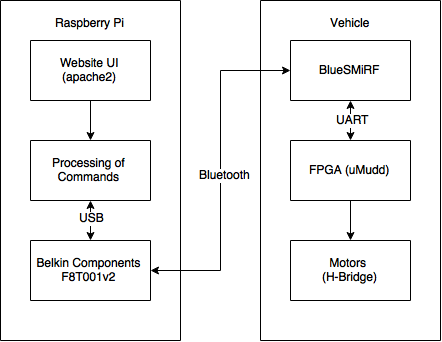
\includegraphics[width=0.7\textwidth]{E155System}
\end{center}
\caption{An overview of the system. The system is comprised of two major subsystems: the Raspberry Pi 2 controller and the vehicle, which is controlled by the $\mu$Mudd board.}
\label{fig:sys}
\end{figure}

The Internet-Controlled Autonomous Ground Vehicle is a treaded chassis that holds an FPGA with bluetooth listening capabilities. A companion website allows a user to interact with the vehicle by commanding it to travel it to various places. The motivation behind this project was to build a tank that could navigate within a map and shoot NERF darts. By building a tank that is remotely controlled over the internet, the more difficult part of this concept is realized.

The project involves a website hosted by Apache2 on the Raspberry Pi 2, which sends commands from the a bluetooth dongle to a bluetooth receiver (BlueSMiRF) that is connected to the FPGA. The FPGA drives two motors. Each component is described further in the following sections.

\section{New Hardware}
\subsection{BlueSMiRF}
The Raspberry Pi and FPGA communicate with each other using a set of Bluetooth modules.  The FPGA is wired to a SparkFun BlueSMiRF module.  The Raspberry Pi has a Belkin FT8001 Bluetooth dongle

The BlueSMiRF is a Bluetooth RF module that has a UART pinout to interface with.  To set up the interface, the device is powered with a single-sided +5V/GND power source, in this case the same 5V output from the voltage regulator and ground line on the breadboard.  RTS and CTS are wired together, and the TX and RX pins on the BlueSMiRF are connected to the pins of the FPGA that are assigned to RX and TX, respectively. (how to find address and how to config)

The Belkin FT8001 is a USB Bluetooth dongle that can be attached directly to the Raspberry Pi's USB port. (how to config)

To power the vehicle, the FPGA's H-Bridge outputs 1/2 and 3/4 are connected to two Pololu Brushed DC motors.  The motors operate at 3-12V volts, which allows the same voltage regulator to power the input of the FPGA and the motors.
\subsection{Vehicle}

The vehicle is a Tamiya Tracked vehicle modified to accept a double gear box. The motors are wired directly to the H-Bridge outputs. The battery case is wired directly to a 5V regulator, which powers the system. The breadboard is mounted on three sheet metal stands.

\section{Schematics}

Figure \ref{fig:breadboard} shows the layout of the breadboard. The two main components are the FPGA and the BlueSMiRF. The 7.4 V power source is comes from two TrustFire 3.7 V batteries, and is regulated with the 5V regulator. The switch makes for easy powering on and off of the vehicle.

\begin{figure}
\begin{center}
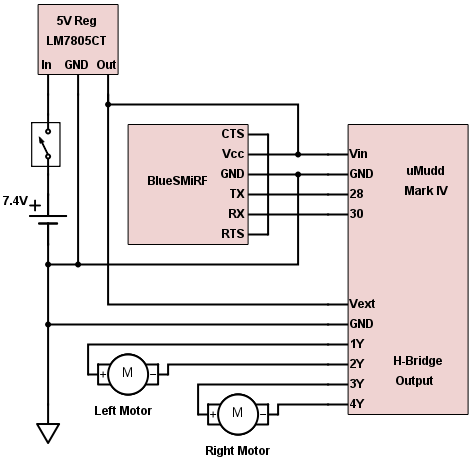
\includegraphics[width=0.7\textwidth]{breadboard}
\end{center}
\caption{The components on the breadboard. The H-Bridge Output are PWM signals.}
\label{fig:breadboard}
\end{figure}

\section{Raspberry Pi}

The Raspberry Pi 2 serves several functions. It hosts an Apache2 website accessible via the internet and contains code to submit commands to a bluetooth dongle. These two functions are integrated such that a user interacts with the website, indirectly sending commands over bluetooth. Figure \ref{fig:piroutines} show the flow of data and control through the Pi.

The languages in use on the Pi are HTML, JavaScript, C, and Python.

\begin{figure}
\begin{center}
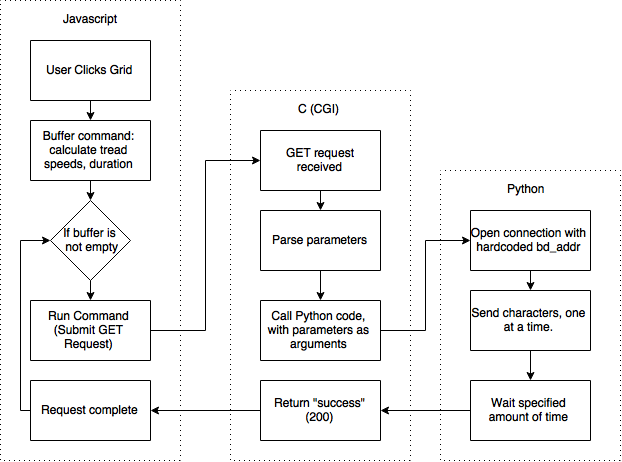
\includegraphics[width=0.8\textwidth]{PiRoutines}
\end{center}
\caption{The flow of control and data through the Pi.}
\label{fig:piroutines}
\end{figure}

\subsection{Website}

The website contains a visual user interface that contains instructions for use, a grid on which to input locations for the robot to maneuver to, a list of the commands currently buffered for sending. The resulting webpage is shown in Appendix \ref{sec:web}, along with the code in Appendix \ref{sec:webcode}. The website was built using HTML, JavaScript, and Bootstrap CSS. 

The Pi hosts the website. Upon clicking in a grid space, the page's JavaScript calculates the left and right tread speeds and duration of movement required to get the tank to move from its original position to the new position. The current algorithm involves first moving north/south, turning, moving east/west, and finally turning to reorient itself vertically. Once the commands are generated, the JavaScript makes an HTTP GET request to the inputChars resource of the Pi. When the request is completed, the page updates, either submitting the next command in the buffer or waiting for another input from the user.

\subsection{Python/C}
After receiving a GET request, the common gateway interface (CGI) reads the input parameters (three integers) and converts them into a format that the vehicle understands. This involves converting the numbers to sign/magnitude bit representations. Because of how the UART works, the C also reverses the bits.

Then, the C program calls a Python script. The Python script utilizes the \verb.bluetooth. module to allow sending data using the bluetooth dongle. When called, the Python script sends the commands, one at a time, to the robot. The system sleeps for the amount of time to give the vehicle enough time to move. The code on the Pi is shown in Appendix \ref{sec:pi}. 

To send data over bluetooth, the address of the BlueSMiRF must be known. This can be done with a scan of all devices in the area. The scan is initiated with the terminal command
\begin{verbatim}
      hcitool scan
\end{verbatim}
Another way to do it is to scan in the Python script and match the name of each device in the area to the device's name. In any case, something has to be hardcoded into the Python script to make a connection with the BlueSMiRF. To save time when connecting to the vehicle, the address is hardcoded and thus there is no need to scan.

Sending data in Python with the \verb.bluetooth. module is fairly simple.

\begin{verbatim}
      sock = BluetoothSocket( RFCOMM )
  
      try:
          sock.connect((bd_addr, port))
      except:
          # Address is likely in use, so close it.
          sock.close()
          return
      
      # Send each character individually
      for c in data:
          sock.send(c)
      
      sock.close()
\end{verbatim}
First a connection is made, data is sent over it, and the connection is closed. This could be done by only connecting once, however the nature of the website and the desired interaction made connecting and disconnecting for each command a simpler and understandable solution.

\section{FPGA Design}

The FPGA reads data from the BlueSMiRF using UART hardware coded in SystemVerilog, processes and executes the command, and then sends an acknowledgment back to the Raspberry Pi.  It is constructed as a controller-datapath pair with three main submodules in the datapath - receiveMSG, executeCommand, and sendAck.  The SystemVerilog code installed on the FPGA is shown in Appendix \ref{sec:fpgacode}. The FPGA and BlueSMiRF are the only two electrical components on the breadboard. Two motors are connected to the $\mu$Mudd board's H-bridge screw terminals.  The schematic is shown in figure.

The clock used to interface with the BlueSMiRF is implemented using a PLL that oversamples the 115.2 Kbaud UART frequency at 921.6kHz, or a factor of 8.  This oversampler determines if there is an incoming message.  The actual sampling of the BlueSMiRF's TX line is accomplished using a frequency divider that allows for sampling at the correct rate.  The divider's phase can be frozen when the start bit has not yet been detected.  This ensures that the sampling of the line is as close to the center of the transmission's clock as possible.  The Raspberry Pi sends three characters, which are flushed by the Bluetooth module's buffer at the same time, so the command appears as a 30-bit message.  The sampler stops sampling when it sees a stop bit, and either begins a new message if the next bit is a start bit, or signals to the controller that a command has been received of an entire command if the line has remained high.

\begin{figure}
\begin{center}
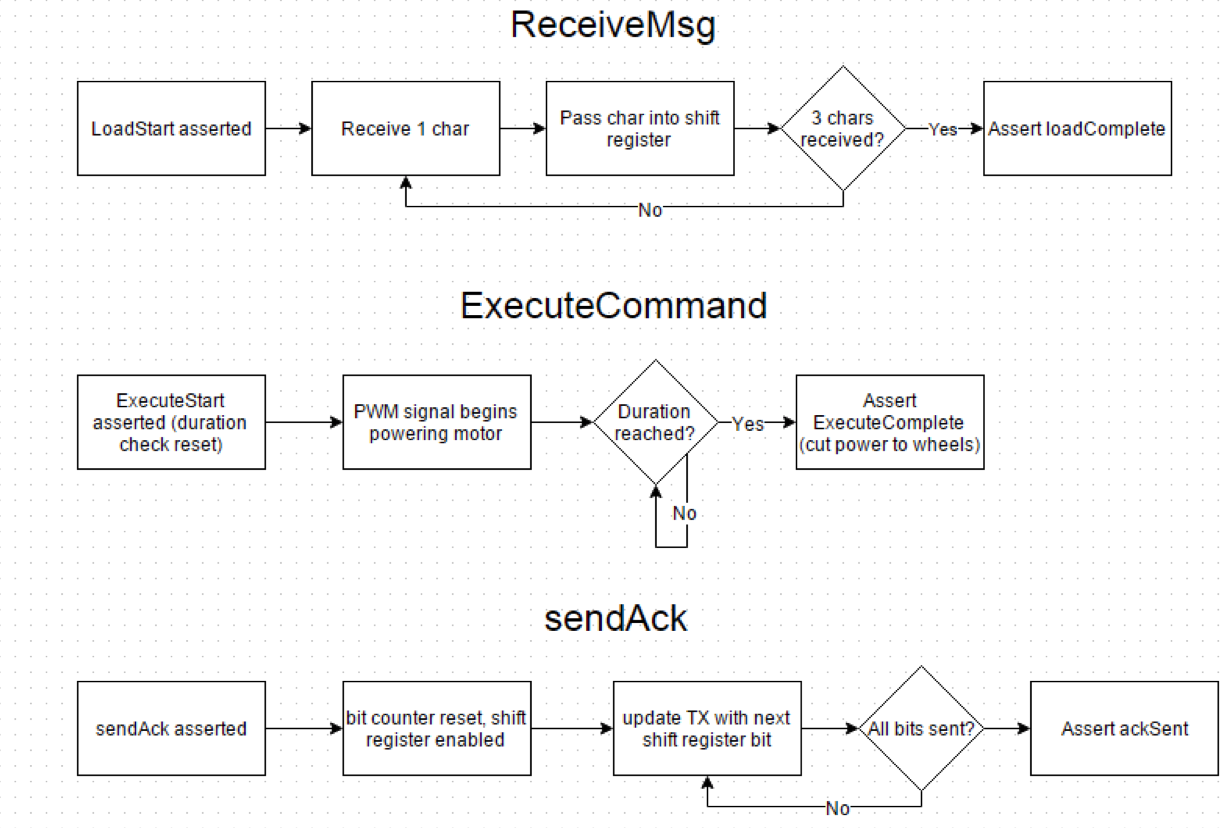
\includegraphics[width=0.8\textwidth]{FPGABlock}
\end{center}
\caption{Schematic overview of the FPGA.}
\label{fig:fpgablock}
\end{figure}

The FPGA executes the command received by controlling the two motors via the H-Bridges on the $\mu$Mudd board. Each command consists of a PWM setting and rotation direction for each motor and a duration for which the motors should be turning.  A counter is used to create a reference clock for PWM; the power levels are referenced against this counter to determine the correct duty cycle.  Multiplexers are used to route the power to the correct pins on the H-Bridge, allowing for both forward and backwards movement.  To prevent the vehicle from running indefinitely, the timer stops incrementing when the requested duration is reached, and a signal is output that is used to cut power to the motors.  Each LSb of the duration character corresponds to roughly one-tenth of a second.

Once the requested duration has been reached and power to the motors cut, the FPGA transmits the character `A' back to the BlueSMiRF as an ACK code.  After this ACK has been sent, the FPGA will return to the receiveMSG state and start to sample for a new command.

A flowchart detailing each state of the FPGA is shown in Figure \ref{fig:fpgablock}.



\section{Results}

The system has met all of the proposals, but does not always meet each one consistently.  There are a few bugs of as-of-yet unidentified origin, most likely in the FPGA's SystemVerilog code, that occasionally cause the system to miss commands or fail to send an ack.  These bugs are not easily reproducible.

As proposed, the Raspberry Pi hosts a website using an apache2 server.  The website contains a grid with clickable cells, each of which correspond to a location on the ground. Clicking the grid triggers Javascript that updates the UI and submits code that calls C code in the cgi-bin.  This C code processes the submission and converts it to the necessary command(s) to be sent to the FPGA, and then calls a Python script to send the data.  The website is then updated with a ``receipt" of the transmission (the HTTP response).  When multiple commands need to be sent, unsent commands fill a queue.  Refreshing the page will clear the buffer.  In addition to what was proposed, the user is able to send arbitrary commands to the FPGA, and can also click on buttons to nudge the robot both rotationally and translationally.

The Raspberry Pi itself is connected to a USB Bluetooth dongle that it can send data to in order to transmit the proper commands to the FPGA.  The C code in the Pi has the ability to wait for an ack before sending the next command.  However, this feature is currently disabled because a bug in the FPGA seems to sometimes cause the system to skip the ack stage in the controller's loop.  Instead, the Pi uses only the timeout for the ack (ack timeout at one second longer than the command's duration) as a signal to send the next command.

The FPGA implements UART in order to communicate with the BlueSMiRF.  Data is clocked out by the BlueSMiRF to the FPGA, where it is read into a series of shift registers, one which is bit-wide for reading the RX line and one which is byte-wide to store the received characters.  Upon completion of the transmission, the FPGA sends the entire contents of the byte-wide shift register to the modules that control the PWM signal and signal routing to the H-Bridge.  The commands that are successfully read from the BlueSMiRF are executed correctly.

The vehicle was built from a kit, but was modified to accept a Tamiya double gearbox.  This allowed for two motors to independently drive the treads of the vehicle.  The motors are wired to the H-Bridge output pins, and the breadboard on which the circuitry is located is supported by sheet metal supports.

%\section{References}
%\renewcommand{\refname}{}
%\vspace{-1cm}
%\begin{thebibliography}{widest entry}
% \bibitem{E102}
%REFERENCES?
%\end{thebibliography}
\section{Parts List}
This is the bill of materials for the project.
\begin{center}
\begin{tabular}{|l|l|l|l|}
\hline
\multicolumn{1}{|c|}{\textbf{Item}} & \multicolumn{1}{c|}{\textbf{Description}}               	& \multicolumn{1}{c|}{\textbf{Source}} & \multicolumn{1}{c|}{\textbf{Cost}} \\ \hline
Tracked Vehicle 			&										&							&	\\
			Chassis Kit	& Chassis for the tank, includes treads and frame.    	& Amazon 					& 15.39                          	\\ \hline
Tamiya 70168				& Gives tank flexibility to turn by controlling each     	& 							& \\
Double Gearbox			& tread independently.						& Amazon		               			& 11.99                             	\\ \hline
$\mu$Mudd Board                	& Controls the vehicle.                                                & E155                                 		& 0.00                               	\\ \hline
			                      	& Provides website interface and sends commands 	&							&\\
Raspberry Pi 2			    	& to vehicle.             							& E155                                 		& 0.00                               	\\ \hline
                        				& Wirelessly communicate via Bluetooth between  	&							&\\
BlueSMiRF				& Pi and $\mu$Mudd board.		 			& E155                                		& 0.00                               	\\ \hline
Belkin Components			&										&							&					\\ 
FT8001					& Send bluetooth data from Pi.					& E155                                		& 0.00                               	\\ \hline
2X TrustFire 14500			& Li Ion battery, 3.7 V 						& Aaron Rosen					& 0.00				\\ \hline
Brushed DC Motor			& Pololu 1117. Size: 130						& Aaron Rosen					& 0.00				\\ \hline
LM 7805 CT				& 5V Regulator						& Stockroom					& 0.00				\\ \hline
\end{tabular}
\end{center}


\section{Appendices}

\subsection{The Website}
\label{sec:web}

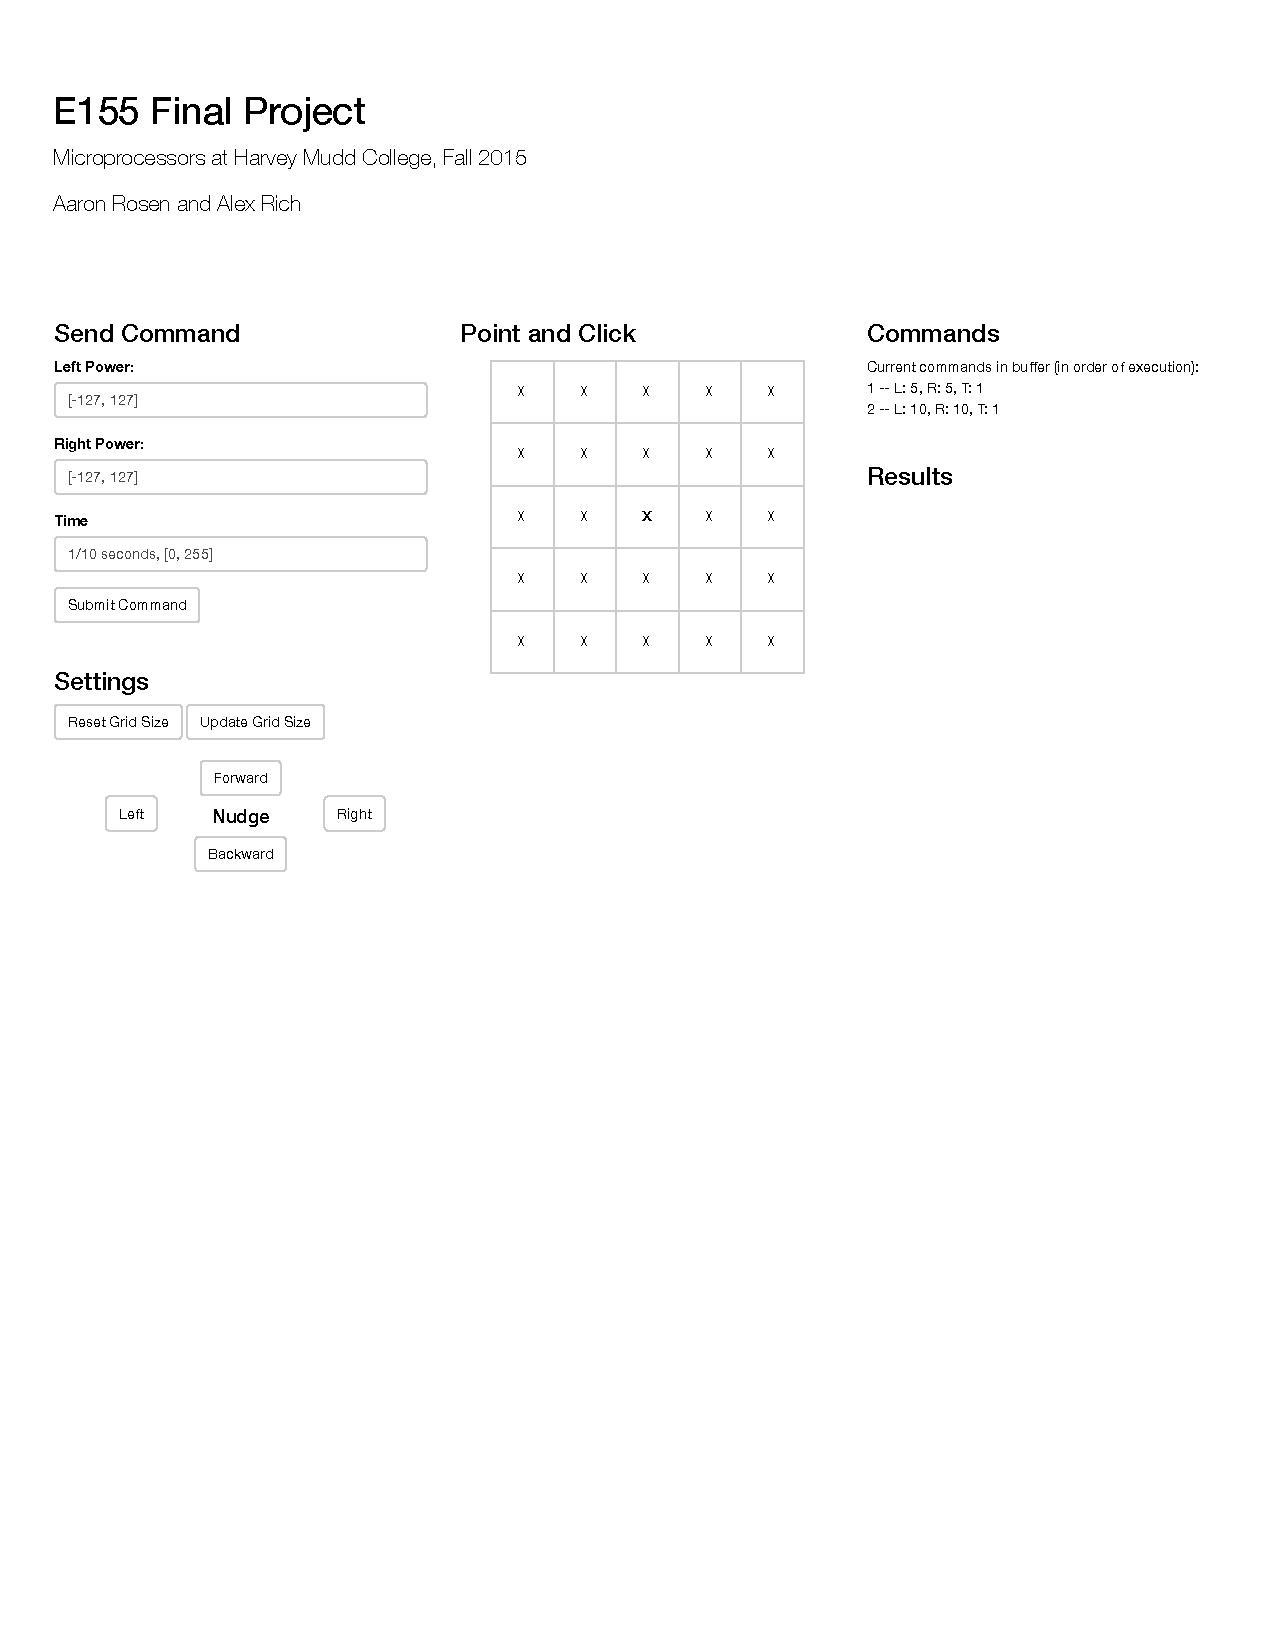
\includegraphics[width=\textwidth]{website}


\subsection{FPGA Diagrams}
\subsubsection{Controller}
\begin{center}
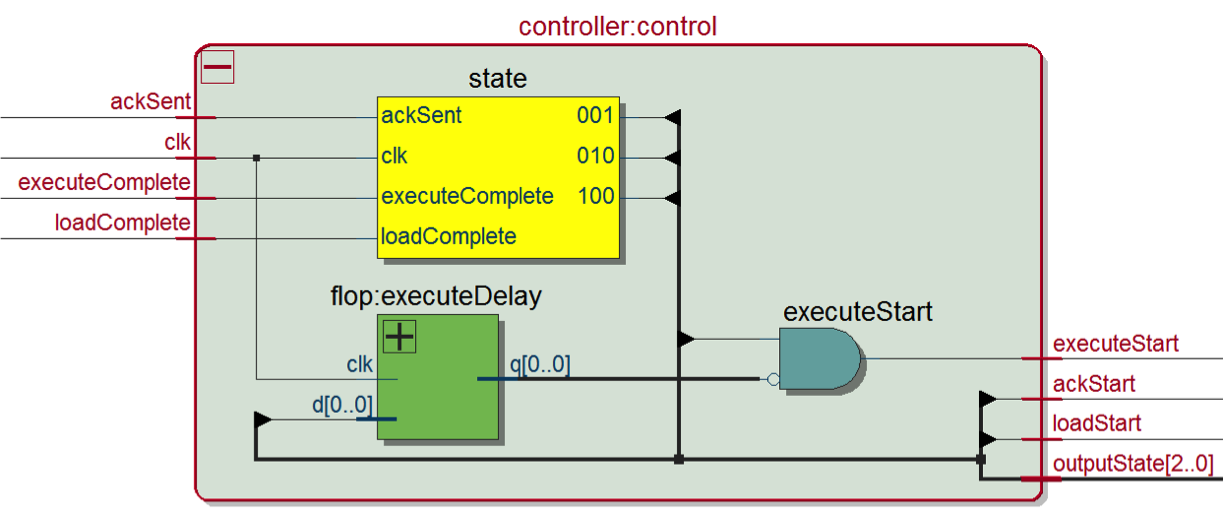
\includegraphics[width=0.8\textwidth]{controller}
\end{center}
\verb.clk. - 40MHz input clock 
\\ \verb.loadComplete. - command loaded
\\ \verb.executeComplete. - successful vehicle travel
\\ \verb.ackSent. - ack sent successfully
\\ \verb.loadStart. - enables reception of commands
\\ \verb.executeStart. - pulse that resets duration timer
\\ \verb.ackStart. - enables sending of ack
\\ \verb.outputState. - output state of FSM (for scope only)

\begin{center}
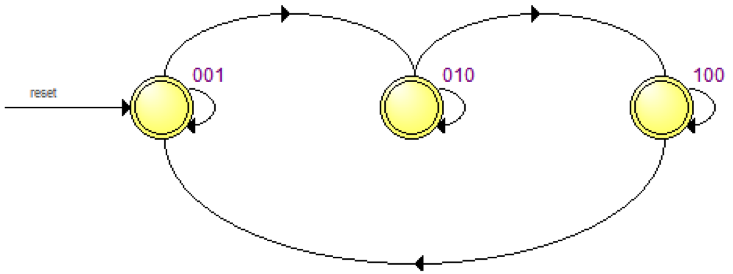
\includegraphics{states}

Controller State Machine
\end{center}




%%%%%
\subsubsection{Receive A Char}
This module reads one 8 bit input from the BlueSMiRF.
\begin{center}
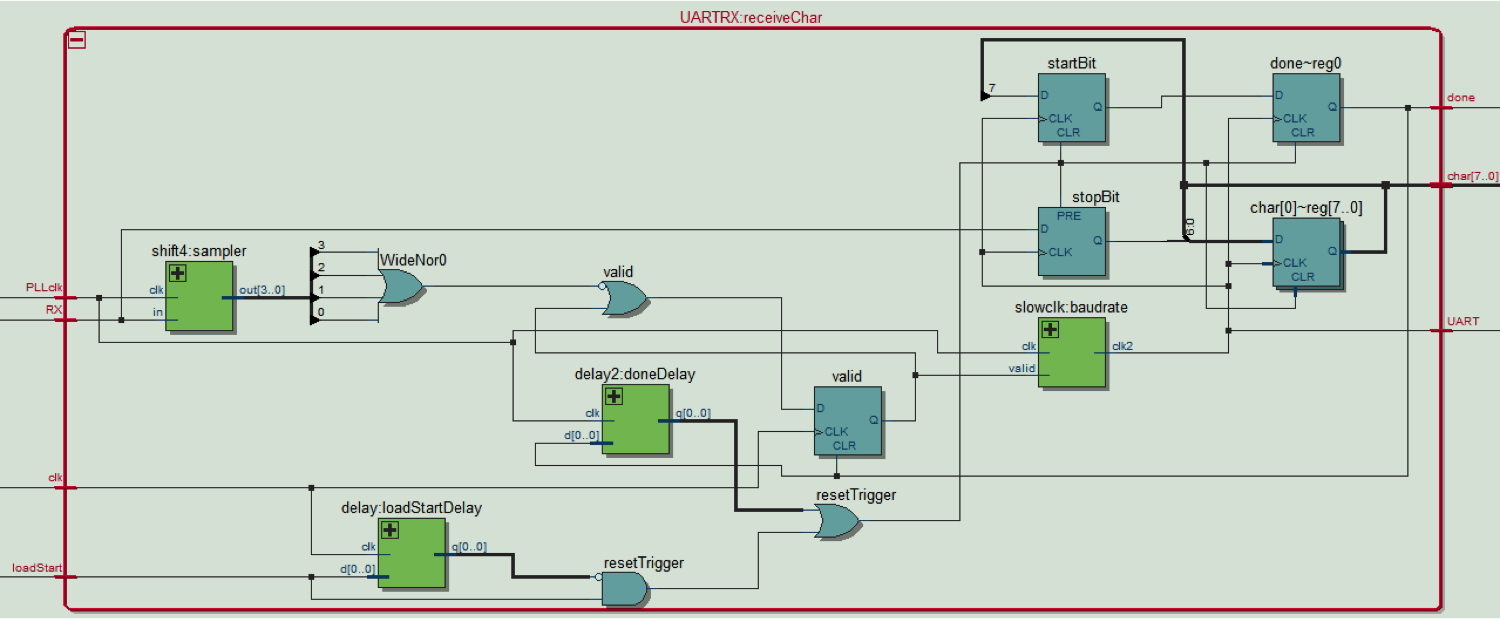
\includegraphics[width=\textwidth]{receiveChar}
\end{center}
\verb.loadStart. - Resets shift register
\\ \verb.clk. - 40MHz input clock
\\ \verb.PLLclk. - 921.6KHz UART oversampler
\\ \verb.RX. - BlueSMiRF TX/ FPGA RX
\\\\ \verb.done. - signals end of char received
\\ \verb.char. - the char received
\\ \verb.UART. - the 115.2KHz clk that samples the FPGA RX line (for scope only)



%%%%%
\subsubsection{Receive A Message}
This module reads three 8 bit inputs from the BlueSMiRF.
\begin{center}
\includegraphics[width=\textwidth]{rxin}
\end{center}
\verb.loadStart. - Enables receiveChar and shift registers
\\ \verb.clk. - 40MHz input clock
\\ \verb.PLLclk. - 921.6KHz UART oversampler
\\ \verb.RX. - BlueSMiRF TX/ FPGA RX
\\\\ \verb.lmotor. - left motor PWM/direction
\\ \verb.rmotor. - right motor PWM/direction
\\ \verb.dur. - command duration
\\ \verb.loadComplete. - signals end of command
\\ \verb.sampler. - UART sampler (for scope only)
\\ \verb.RXdone. - signals end of char received (for scope only)


%%%%%
\subsubsection{Send A Char}
This module sends one 8 bit output to the BlueSMiRF.
\begin{center}
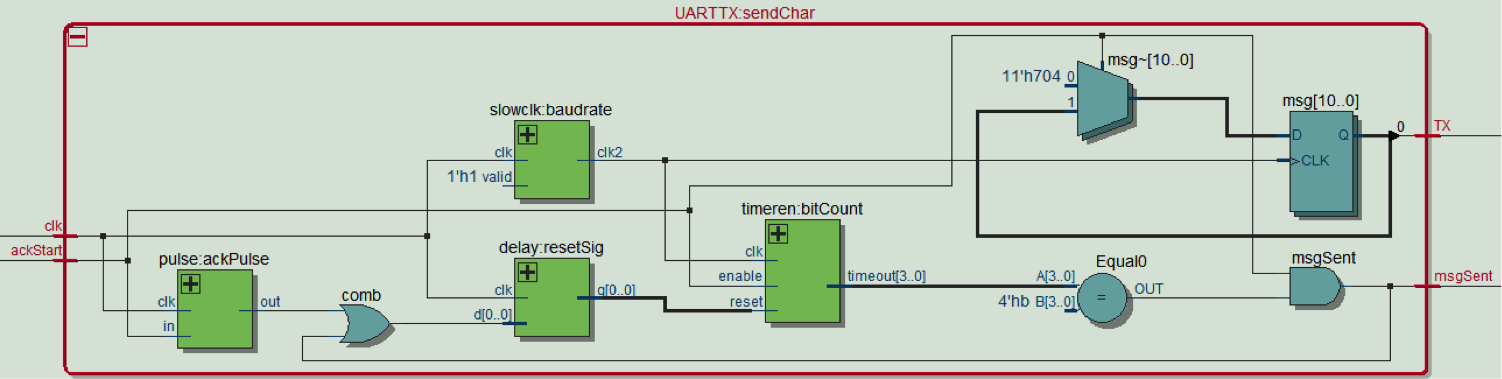
\includegraphics[width=\textwidth]{sendChar}
\end{center}
\verb.clk. - 921.6KHz UART oversampler
\\ \verb.ackStart. - resets counter to begin transmitting ack message
\\\\ \verb.TX. - the FPGA TX / BlueSMiRF RX
\\ \verb.msgSent. - indicates successful transmission of ACK



\subsection{FPGA Code}
\label{sec:fpgacode}
\lstinputlisting[language=Verilog]{VehicleControl.sv}

\subsection{Raspberry Pi Code}
\label{sec:pi}

\subsubsection{CGI Resource}
\lstinputlisting[language=C]{inputChars.c}

\subsubsection{Send Data over Bluetooth}
\lstinputlisting[language=Python]{sendData.py}

\subsubsection{Webpage}
\label{sec:webcode}
\lstinputlisting[language=html]{final.html}


\end{document}
